\section{梯度提升决策树}
\subsection{分类与回归树}
%1. 分类与回归树\par
	我们之前已经学习了决策树。决策树常常被用于分类任务,但是,有没有可能将决策树用作回归任务呢?\par
	在上一章的决策树例子中,决策树的每个叶子节点都有一个输出的分类。如果叶子节点的输出值不再是某个分类,而是一个实数值,就可以将决策树用于回归任务。实际上,一棵决策树就是将输入空间划分成了许多区域,每个区域对应一个输出值。如果输出值是一个分类,就可以被用作分类任务;如果是实数值,则可被用作回归任务。用作回归任务时,只要划分出的区域足够小,就可以用区域中样本点的平均输出值近似地代替真实的输出值。\par
	Breiman等在1984年提出的分类与回归树(Classification And Regression Tree, CART)就是一种像上面一样的决策树,分为分类树和回归树两种。CART的学习算法有生成和剪枝两步。\par
%	A. 分类树生成\par
\subsubsection{分类树生成}
	首先引入基尼指数(Gini index)作为选择最优二分的指标。基尼指数反映了数据集中随机抽取的两个样本的分类不一致的概率,其定义如下:\par
\begin{equation}
	Gini(D)=\sum\limits_{k=1}^K p_k(1-p_k)=1-\sum\limits_{k=1}^K p_k^2
\end{equation}
	其中,数据集$D$有$K$个类,第$k$类样本的频率为$p_k$。\par
	特别地,当数据集$D$中只有两类且其中一类的频率为$p$时,
\begin{equation}
	Gini(D)=2p(1-p)
\end{equation}
	若数据集$D$根据特征$A$是否有$A=a$被分成子集$E, F$,则其基尼系数定义为
\begin{equation}
	Gini(D,a)=\frac{|E|}{|D|}Gini(E)+\frac{|F|}{|D|}Gini(F)
\end{equation}
	其中$|D|$表示集合$D$的元素个数。\par
\begin{algorithm}  
\caption{CART分类树生成算法}
\begin{algorithmic}[1]
\Require 训练集$D$,停止计算的条件
\Ensure 一棵CART分类树
	\State 新建节点$N$,其左右子节点分别为$L,R$
	\State 对每个特征$S$的可能取值$a$,根据是否有$A=a$将数据集$D$分为两个子集,并计算分割后的基尼系数$Gini(D,a)$
	\State 选择基尼系数最小的分法,得到子集$E,F$。
	\State $L$=CART分类树生成算法($E$,停止计算的条件)
	\State $R$=CART分类树生成算法($F$,停止计算的条件)
	\State 返回$N$
\end{algorithmic}  
\end{algorithm}  
\subsubsection{回归树生成}
%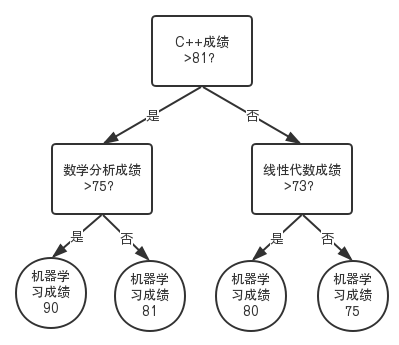
\includegraphics[width=\textwidth]{regression_tree.png}\par
\begin{figure}[htbp]
	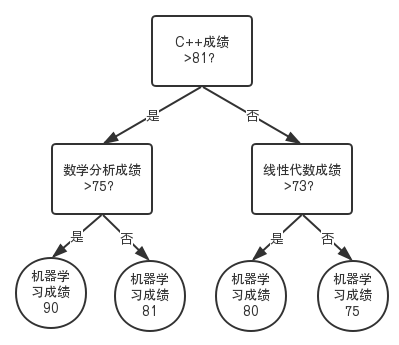
\includegraphics[width=\textwidth]{regression_tree.png}
	\caption{回归树示例}
	\label{reg_tree}
\end{figure}
	假设数据集的输入输出变量均为连续值,设数据集$D=\{(x_1,y_1),(x_2,y_2),...,(x_n,y_n)\}$\par
	设输入空间被划分为区域$R_1,R_2,...,R_m$,每个区域$R_i$有一个固定的输出值$c_i$,则回归树可表示为
\begin{equation}
	f(x)=\sum\limits_{i=1}^m c_i I(x \in R_i)
\end{equation}
	回归树使用平方误差$\sum\limits_{x_j \in R_i} (y_j - f(x_j))^2$作为每个区域$R_i$的预测误差。若要令预测误差最小,易知,在区域$R_i$上,$c_i$为$R_i$中所有样本点的平均输出值,即
\begin{equation}
	c_i=mean(y_j | x_j \in R_i)
\end{equation}
	显然,$R_i$上的最小预测误差为输出值的方差。\par
	在回归树生成的每一步上,为了对输入空间进行划分,将数据集分成两个子集,需要选择第$k$个变量$x^{(k)}$及其取值$s$,作为切分变量(splitting variable)和切分点(splitting point),将输入空间分割为两个区域
\begin{equation}
	L(k,s)=\{x|x^{(k)}\leq s\}
\end{equation}
	和
\begin{equation}
	R(k,s)=\{ x|x^{(k)}>s\}
\end{equation}\par
	求解
\begin{equation}
	(k_*,s_*)=\mathop{\arg\min}\limits_{(k,s)}(var(y_i|x_i\in L(k,s))+var(y_i|x_i\in R(k,s)))
\end{equation}
	可得当前输入空间的最优切分变量和最优切分点。\par
	对每一个叶子节点重复以上步骤,直到满足停止条件为止,即可生成一棵回归树。\par
\begin{algorithm}
\caption{CART回归树生成算法}
\begin{algorithmic}[1]
\Require 训练集$D$,停止条件
\Ensure 一棵CART回归树
	\State 遍历$k=1,2,...,n$,求解$(k_*,s_*)=\mathop{\arg\min}\limits_{(k,s)}(var(y_i|x_i\in L(k,s))+var(y_i|x_i\in R(k,s)))$,将训练集$D$分成两个子集$E,F$。
	\State 重复以上步骤,直到满足停止条件为止。
\end{algorithmic}
\end{algorithm}
\subsubsection{剪枝}
	剪枝算法由两步组成:第一步,将CART决策树$T_0$从叶子节点开始不断剪枝,直到根节点,每剪一次输出一棵决策树,形成一个决策树序列$\{ T_0,T_1,...,T_n\}$;然后通过交叉验证法用独立的验证集选出最优的决策树。\par
	给出子树的损失函数
\begin{equation}
	C_\alpha (T)=C(T)+\alpha |T|
\end{equation}
其中,$T$为任意子树,$C(T)$为对训练数据的预测误差(如基尼指数),$|T|$为子树的叶子节点个数,$\alpha \ge 0$为参数,用于权衡拟合程度和模型复杂度。\par
	对于内部节点$t$,剪去以$t$为根节点的子树$T_t$(会留下节点 )的临界值$\alpha$可由$C_\alpha (T_t)=C_\alpha (t)$解得。可知
\begin{equation}
	\alpha=\frac{C(t)-C(T_t)}{|T_t|-1}
\end{equation}
	对于每个内部节点$t$,设
\begin{equation}
	g(t)=\frac{C(t)-C(T_t)}{|T_t|-1}
\end{equation}
作为$\alpha$的不同取值下剪枝的依据。当$\alpha \ge g(t)$时,即可对$t$剪枝。\par\
	求出每个内部节点的$g(t)$,每次取最小的$g(t)$值进行剪枝,得到剪枝后的决策树序列$\{ T_1,T_2,...,T_n\}$。\par
	生成决策树序列$\{ T_0,T_1,...,T_n\}$后,对每棵树用验证集测试,选出平方误差或基尼指数最小的作为最优决策树$T_\alpha$。\par
\begin{algorithm}
\caption{CART剪枝算法}
\begin{algorithmic}[1]
\Require CART算法生成的决策树$T_0$,测试集$D_T$
\Ensure 最优决策树$T_\alpha$
	\State 计算出每个内部节点的$g(t)$值。
	\State 根据从小到大的$g(t)$值对$T_i$进行剪枝,得到$\T_{i+1}$,直到得到决策树序列$\{T_0,T_1,...,T_n\}$。
	\State 使用测试集$D_T$选出最优决策树$T_\alpha$
\end{algorithmic}
\end{algorithm}
\subsection{梯度提升(Gradient Boosting, GB)}
%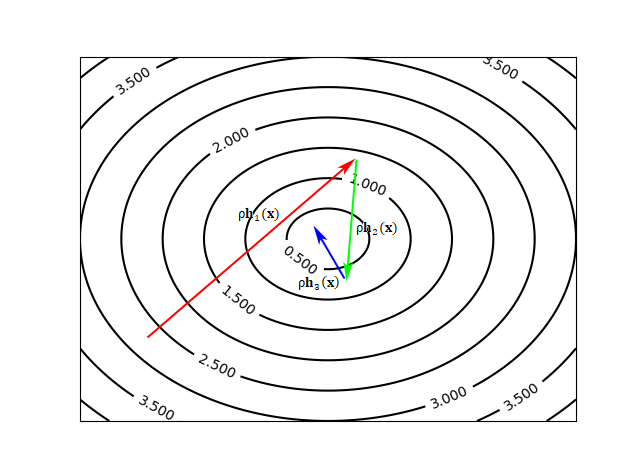
\includegraphics[width=\textwidth]{gb.png}\par
%\begin{figure}
%	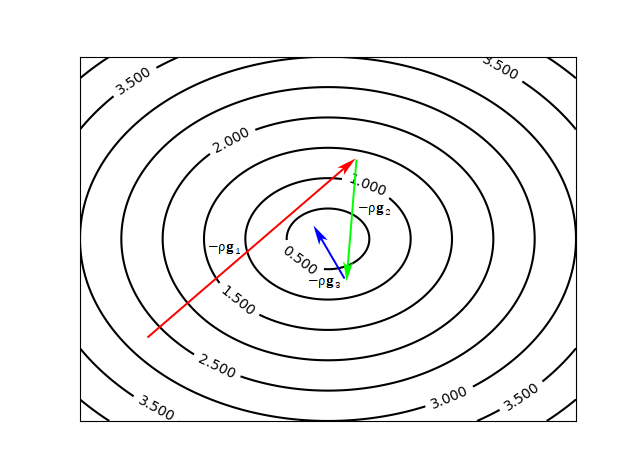
\includegraphics[width=\textwidth]{gd2.png}
%	\caption{梯度下降}
%\end{figure}
%\hfill
%\begin{figure}
%	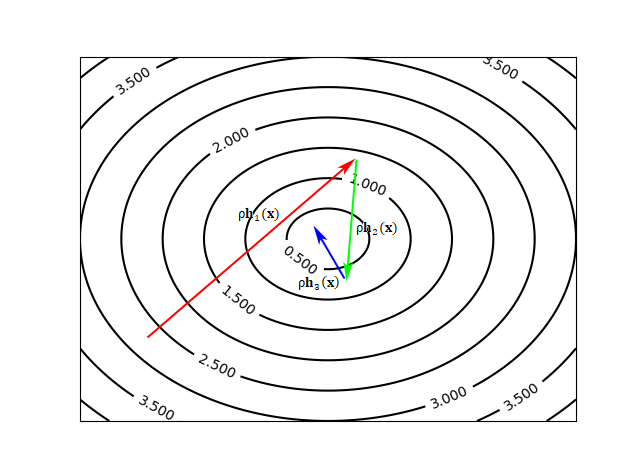
\includegraphics[width=\textwidth]{gb.png}
%	\caption{梯度提升}
%\end{figure}
\begin{figure}[htbp]
	\begin{minipage}[t]{0.4\linewidth}
		\centering
		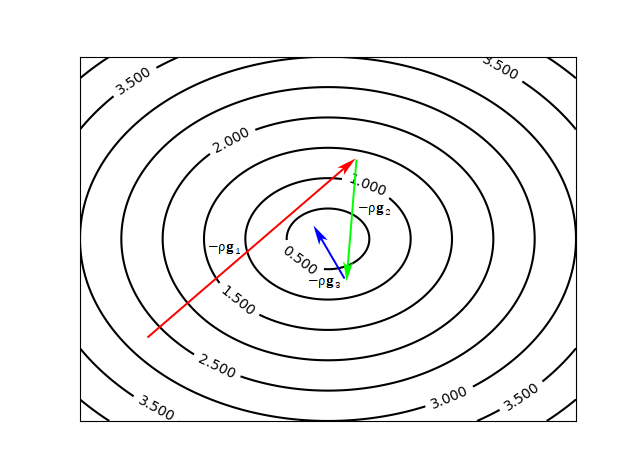
\includegraphics[width=\textwidth]{gd2.png}
		\caption{梯度下降}
	\end{minipage}
	\hfill
	\begin{minipage}[t]{0.4\linewidth}
		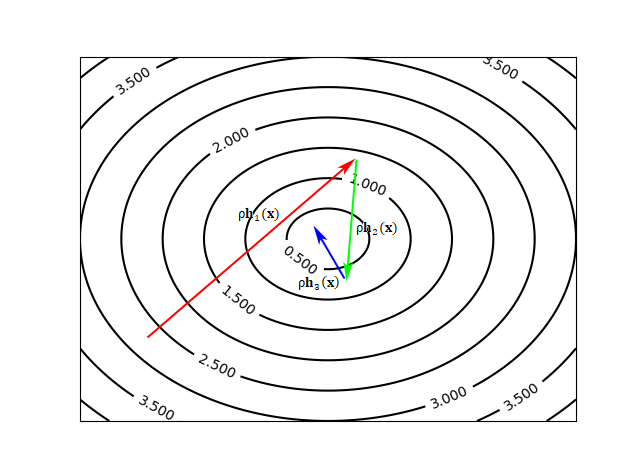
\includegraphics[width=\textwidth]{gb.png}
		\caption{梯度提升}
	\end{minipage}
\end{figure}
	在梯度下降法中,通过将变量往损失函数梯度的负方向不断修正,我们最终得到了数值解。那么,如果我们将弱学习器得到的预测结果也往损失函数梯度的负方向不断修正,是不是也能得到一个更接近真实值的预测结果呢?\par
	但是,梯度下降法要修正的是一个数值解,其在算法结束后就不会再改变,是一个常量;而梯度提升则需要考虑到不同的输入值,要修正的是一个与输入值有关的变量。所以,这里的梯度是要随着输入值而改变的。如果可以确定修正预测结果的梯度与输入值相关,我们就可以用弱学习器预测不同输入值下的梯度。\par
	对于损失函数$l(y,\hat{y})$,预测值和真实值都是与$x$相关的,所以其梯度也是与$x$相关的。\par
	设有数据集$D=\{(x_1,y_1),(x_2,y_2),...,(x_n,y_n)\}$和单个损失函数$l(y,\hat{y})$。不妨设初始预测函数
\begin{equation}
	F_0(x)=0
\end{equation}\par
	考虑$j=1,2,...,m$,对于第$j$步,上一步得到预测函数$F_{j-1}(x)$,使用函数$f(x)=F_{j-1}(x)$预测$y$的损失为
\begin{equation}
	L_f=\sum\limits_{i=1}^n l(y_i,f(x_i))
\end{equation}\par
	求上式的极小值,可以看作$\hat{u}=\mathop{\arg\min}\limits_u L(u)$。其中,
\begin{equation}
	u=(f(x_1),f(x_2),...,f(x_n))
\end{equation}
\begin{equation}
	L(u)=\sum\limits_{i=1}^n l(y_i,u^{(i)})
\end{equation}
$u^{(i)}$为$u$的第$i$维分量。\par
	求梯度得
\begin{equation}
	\frac{\partial L}{\partial u}=(g_1,g_2,...,g_n)
\end{equation}
其中,
\begin{equation}
	g_i=\left.\frac{\partial l}{\partial\hat{y}}\right|_{\hat{y}=u_{(i)},y=y_i}
\end{equation}\par
	使用弱学习器$h_j(x)$学习负梯度分量$-g_i$关于$x_i$的变化,得$-g=h_j(x)$。然后,求参数
\begin{equation}
	\rho_j=\mathop{\arg\min}\limits_\rho (u+\rho h)
\end{equation}
其中,
\begin{equation}
	h=(h_j(x_1),h_j(x_2),...,h_j(x_n))
\end{equation}
得到该步的预测函数
\begin{equation}
	F_j(x)=F_{j-1}(x)+\rho_j h_j(x)
\end{equation}\par
	实际上,梯度提升可以看做各个弱学习器的线性组合。\par
\begin{algorithm}
\caption{梯度提升算法}
\begin{algorithmic}[1]
\Require 训练集$D=\{(x_1,y_1),(x_2,y_2),...,(x_n,y_n)\}$
\Ensure 梯度提升的一个学习器
	\State 令$F_0(x)=0$
	\For {$j=1,2,...,m$}
		\State $u=(F_{j-1}(x_1),F_{j-1}(x_2),...,F_{j-1}(x_n))$
		\For{i=1,2,...,n}
			\State $g_i=\left.\frac{\partial l}{\partial\hat{y}}\right|_{\hat{y}=u_{(i)},y=y_i}$
		\EndFor
		\State 用数据集$\{(x_1,-g_1),(x_2,-g_2),...,(x_n,-g_n)\}$训练弱学习器$h_j(x)$
		\State $h=(h_j(x_1),h_j(x_2),...,h_j(x_n))$
		\State 求$\rho_j=\mathop{\arg\min}\limits_\rho (u+\rho h)$
		\State 得到$F_j(x)=F_{j-1}(x)+\rho_j h_j(x)$
	\EndFor
	\State 输出学习器$F_m(x)=\sum\limits_{j=1}^m \rho_j h_j(x)$
\end{algorithmic}
\end{algorithm}
	特别地,令$\rho_j=1$,$l(y,\hat{y})=\frac{1}{2}(y-\hat{y})^2$,弱学习器为回归树,得到提升树(boosting tree)算法。此时,$g_i$为残差。\par
\subsection{梯度提升决策树(Gradient Boosting Decision Tree, GBDT)}
	使用回归树作为梯度提升中的弱学习器,即可得到梯度提升决策树。\par
	具体算法可参照梯度提升算法。\par
